\documentclass[11pt]{article}

\usepackage[margin=1in]{geometry}
\usepackage[utf8]{inputenc}
\usepackage{booktabs}
\usepackage{array}
\usepackage{graphicx}
\usepackage{amsmath}
\usepackage{float}
% lmodern: scalable Type1 faces at every size. Without it microtype's font
% expansion aborts with "auto expansion is only possible with scalable fonts"
% as soon as the document uses a size that ships only as a bitmap (footnotes).
\usepackage{lmodern}
\usepackage[T1]{fontenc}
\usepackage{microtype}
\usepackage[hidelinks]{hyperref}
\usepackage{xcolor}

\setlength{\parskip}{0.35em}
\setlength{\parindent}{0pt}

% Sections are numbered; the short subsection titles inside "What we found"
% are not (the paper deliberately avoids 4.1/4.2-style cross-references).
\setcounter{secnumdepth}{1}

% Marker used by `build.py --draft` for a statistic whose data has not landed.
\newcommand{\missingnum}[1]{\textcolor{red}{\textbf{[[#1]]}}}
\newcommand{\doi}[1]{doi:\href{https://doi.org/#1}{#1}}

\title{\bfseries Gender Bias in Automated Hiring\\ --- the Case for De-Identification}
\author{Vasyl Rakivnenko}
\date{Draft}

\begin{document}
\maketitle

% ============================================================================
% This .md file is the SOURCE of the paper. Edit the prose freely.
% Build it with:   python3 build.py     (writes main.tex, main.pdf, and the zip)
% Conventions:  *italic*  **bold**  "quotes"  `code`  [@citekey]
%               # Section   ## Subsection   ### Run-in heading
% Blocks fenced as ```latex (tables, figures, references) are raw LaTeX:
% they pass through untouched -- leave them alone unless you know LaTeX.
%  are editorial notes; build.py strips them.
%
% NUMBERS ARE NEVER TYPED BY HAND. Every statistic is a \{\{PLACEHOLDER\}\} that
% build.py substitutes from results/*.json via numbers.json. An unresolved
% placeholder FAILS the build (use `python3 build.py --draft` to see the PDF
% anyway, with the gaps marked in red). To add a number: put the placeholder
% here and an entry in numbers.json. Never paste a value into the prose.
%
% HOUSE STYLE (the author's brief): readable by a non-technical reader.
% Sentences <= 25 words. One idea per paragraph, <= 6 sentences. No formulas
% in the body. Every number gets its plain meaning inline.
% ============================================================================

\begin{abstract}
\noindent

Hiring tools increasingly sort applicants automatically. A retriever pulls plausible resumes from a large pool. A re-ranker then puts them in final order. We audited 14 commercial and open-source re-rankers with counterfactual pairs: texts identical except for the candidate's name and pronouns. All 14 favored men more often for male-typed jobs than for female-typed ones. Which way a model leans by default is a property of that product, and cannot be known without testing it. In a simulated pool of 20 equally qualified candidates, one common pipeline gave men 79\% of shortlist places, about four in every five. Removing names and pronouns before scoring removes the difference, because it removes the only thing that differs. Half-measures do not: deleting names alone leaves the direction almost perfectly consistent. We argue that de-identification is a cheap, auditable, less discriminatory alternative that deployers should be expected to adopt.

\end{abstract}

\section{Why this matters}

Software that sorts job applicants usually works in two steps \cite{nogueira2019}. A \emph{retriever} scans a large pool and pulls out a few dozen plausible candidates. A \emph{re-ranker} then reads each one against the job description and fixes the final order. The retriever is the clerk who pulls a stack of files; the re-ranker is the decision-maker who reads them and arranges them best-first. The people at the top of that order get looked at. The rest, in practice, do not.

This is not hypothetical. LinkedIn Recruiter returns a ranked list of candidates \cite{linkedin}; the same ranking technology runs the job-seeker side of the market at Indeed and Google \cite{indeed,google}. Published resume-matching systems score a job description and a candidate document together, using the same family of neural rankers we audit \cite{shpjf,confit}.

Researchers have shown that the embedding models behind the retriever carry gender bias \cite{caliskan2017,rakivnenko2024,wilson2024}. The re-ranker has been studied far less, and in a different way: no prior audit scores identical candidates across commercial ranking products. That is the wrong way round. The re-ranker has the last word, and it decides who appears at the top of the recruiter's screen.

Gender bias in neural rankers is not new. Rekabsaz and Schedl showed that BERT rankers surface more male-oriented passages than keyword search for neutral queries \cite{rekabsaz2020}, and later added an adversarial fix \cite{rekabsaz2021}. Both papers ask what the retrieved text is about, not how two candidates who differ only by sex are scored. Audits of language models do ask that, and they disagree on direction. One study of large language models scoring resumes finds an advantage for women \cite{an2025}; an embedding-based resume screener favors male-associated names \cite{wilson2024}. We run the counterfactual test on the re-rankers that commercial hiring stacks actually use, and follow it through to who makes the shortlist.

Two legal regimes already cover this ground. In the United States, a neutral-looking practice that screens out one sex at a disproportionate rate is unlawful unless the employer shows business necessity. Even then it fails if a less discriminatory alternative exists and the employer declines it. In the European Union, systems that filter job applications are classed as high-risk. From December 2027, the organisations that deploy them owe duties to control that risk. Both regimes ask the same practical question: is there a cheaper, fairer way to do the same job?

\section{What we did}

Our test is a counterfactual pair: two versions of the same professional document. They are identical word for word, except for the candidate's name and pronouns. Any difference in score must therefore come from gender, because nothing else differs. We built these documents from 4 templates across 52 occupations. We varied 10 common American given names of each sex, taken from national birth-name records \cite{ssa2026}. We used 4 ways of phrasing the search. That yields 8,320 counterfactual pairs per model. The appendix shows the templates, the query forms, and the name pairs in full.

We scored 82 occupations, then labeled each by the share of women employed in it, from the federal labor-force survey \cite{bls2025}. 30 occupations had no usable labor-force figure -- no matching category, a suppressed estimate, or a share too close to the 30\% and 70\% cutoffs to call -- and are excluded from every number in this paper; the appendix lists all of them, with the reason for each. Of the remaining 52, 18 are male-typed, 21 are female-typed, and 13 are close to evenly split. The evenly split group carries most of the legal weight, because nobody can claim those jobs require a particular sex.

We scored every counterfactual pair with 14 re-rankers, both commercial and open-source. Some models return coarse scores that give the two documents exactly the same number. We count those ties as ties. The tables report them in their own column; where we need a single share, a tie counts as half a win for each document. The appendix lists every model, its vendor, and its tie rate.

To see what this does in practice, we simulated a pool of candidates for one job. It holds 20 documents, half with men's names and half with women's, identical in every other respect. Because the candidates are by construction equally qualified, a fair system should treat them interchangeably. We ran the pool through a common open-source pipeline -- the retriever BAAI/bge-large-en-v1.5 feeding its top 10 candidates to the re-ranker BAAI/bge-reranker-v2-m3 -- and recorded who made the top three. Finally, we re-scored everything after stripping gender markers, at several strengths, to see which strengths actually work.

\section{What we found}

\subsection{Identical candidates are not scored equally}

All 14 models favored the man more often for male-typed jobs than for female-typed ones. The size of that gap varies; its direction never does. For male-typed jobs the median model favored the man in 79\% of comparisons, about four in every five. For female-typed jobs the median model favored the man in only 37\%. Nothing changed between the two documents but the name and the pronouns. The tilt is not random. It follows the same stereotype that would be unlawful in a human screener.

Where a model sits by default is a different matter. On jobs the labor market splits evenly, the median model favored the man in 63\% of comparisons, about three in every five. But the models themselves disagree: 10 of the 14 lean toward men on those jobs, and 4 lean the other way. A buyer therefore cannot guess which sex a given product disadvantages. The direction is invisible from the outside, and knowable only by testing.

\begin{figure}[tbp]
\centering
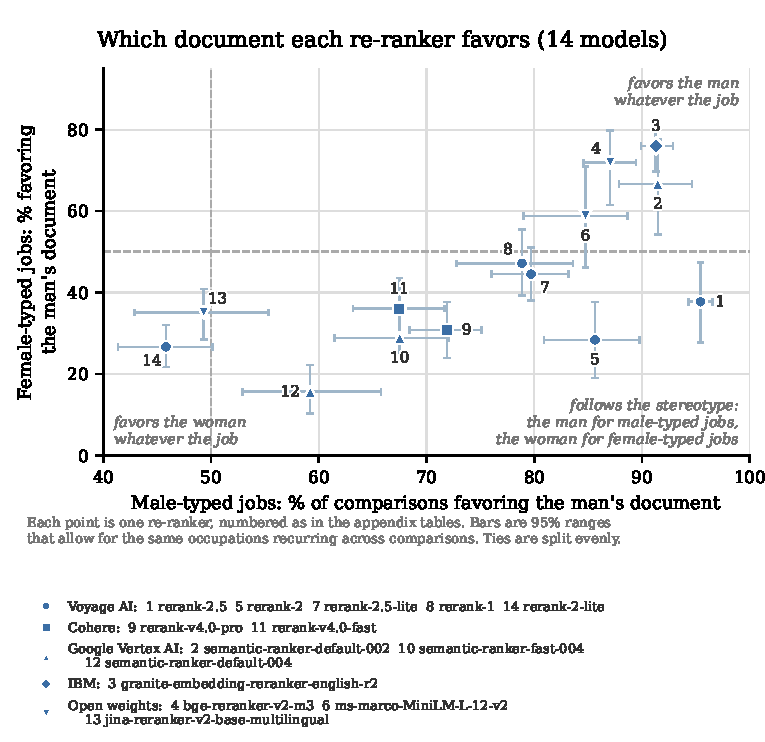
\includegraphics[width=0.78\linewidth]{figures/fig_single_stage.pdf}
\caption{Each point is one re-ranker: how often it favored the man's document
for male-typed jobs (horizontal) against how often it favored the man's document
for female-typed jobs (vertical). A model that treated the pair alike would sit
at 50\% on both axes. Points are numbered as in the appendix tables, and the marker
shape gives the vendor. Where a model scored the two documents exactly equal we split the
tie evenly rather than crediting either side. Bars show the 95\% range across
occupations.}
\label{fig:single}
\end{figure}

\subsection{The re-ranker has the last word}

A pool of 20 interchangeable candidates should produce a shortlist that is half men and half women. It does not. We expected the two stages to compound. A candidate must clear both, so two filters leaning the same way should skew the shortlist further than either alone. That is what happens where they do lean together. On male-typed jobs the retriever alone gave men 76\% of the top three places, the re-ranker alone 90\%, and the two in sequence 95\% -- worse than either stage on its own.

Where the two stages disagree, the effect reverses. On female-typed jobs the retriever leans the other way, giving men 45\% of shortlist places. That pulls the pipeline back from the re-ranker's 70\% to 67\%. Across all jobs the two effects cancel, and the pipeline comes to resemble the re-ranker alone: 79\% against 79\%. For the evenly split jobs it is 77\%.

Favoring either sex among interchangeable candidates is a disparity, so none of these figures is the right answer. Two lessons follow. The pipeline cannot be read off either stage alone; what matters is whether the two happen to agree. And fixing the retriever achieves little on its own, because the re-ranker has the last word.

\begin{figure}[tbp]
\centering
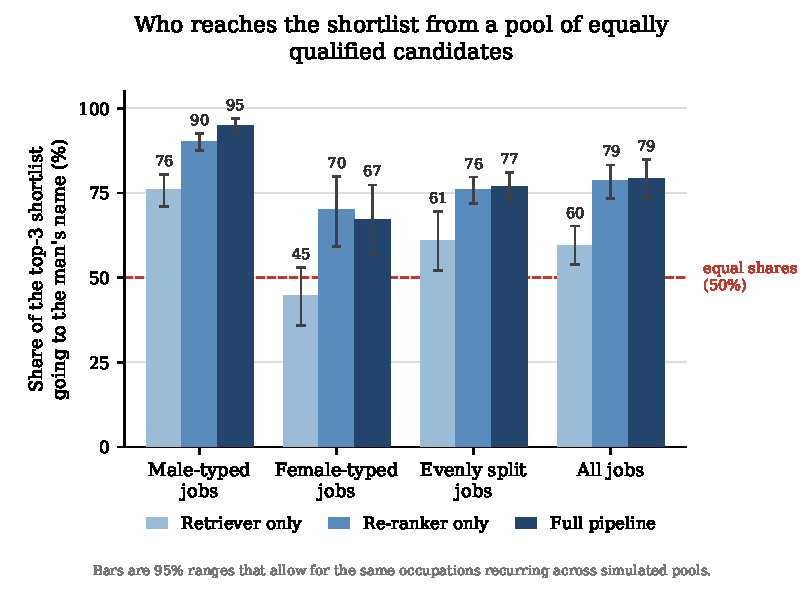
\includegraphics[width=0.82\linewidth]{figures/fig_pipeline.pdf}
\caption{Share of top-three shortlist places going to men's names, in a pool of
equally qualified candidates: under the retriever alone, the re-ranker
alone, and the two combined.}
\label{fig:pipeline}
\end{figure}

\subsection{Removing the markers removes the gap, if you remove all of them}

If both documents become the same text, any model must score them the same. Our full transform replaces the name and neutralises the pronouns, and every pair then ties. That is a check on the argument rather than a discovery, because identical texts cannot be scored differently. Half-measures are the interesting case, and they cut the other way from what you might guess.

Deleting names but leaving pronouns does not shrink the score gap -- if anything it is slightly larger: 0.038 against 0.036. What changes is consistency: the man's document wins 98.6\% of male-typed comparisons, up from 87\%. Removing the name does not take away a large signal and leave a small one behind. It takes away the noisier signal and leaves the more consistent one. Neutralising pronouns but keeping the name shows the same thing from the other side: the gap falls to 0.024. This pattern is not identical on every re-ranker we tested; the appendix repeats it on three more.

So a half-transform is not half a fix. The obvious repair, rewriting pronouns as \emph{they}, \emph{them}, and \emph{their}, works only if the rewriter understands grammar. English \emph{her} is both possessive and object, so mapping it to one word leaves the pair differing by a word. That happens on 25\% of pairs, and where it happens 96\% of the leftovers favor the woman's document, not the man's. A rewriter that checks each word's part of speech avoids the mistake and keeps the text readable. Neither route costs accuracy: the right candidate came out on top 99.8\% of the time, slightly more often than the 99.4\% before any transform.

\begin{figure}[tbp]
\centering
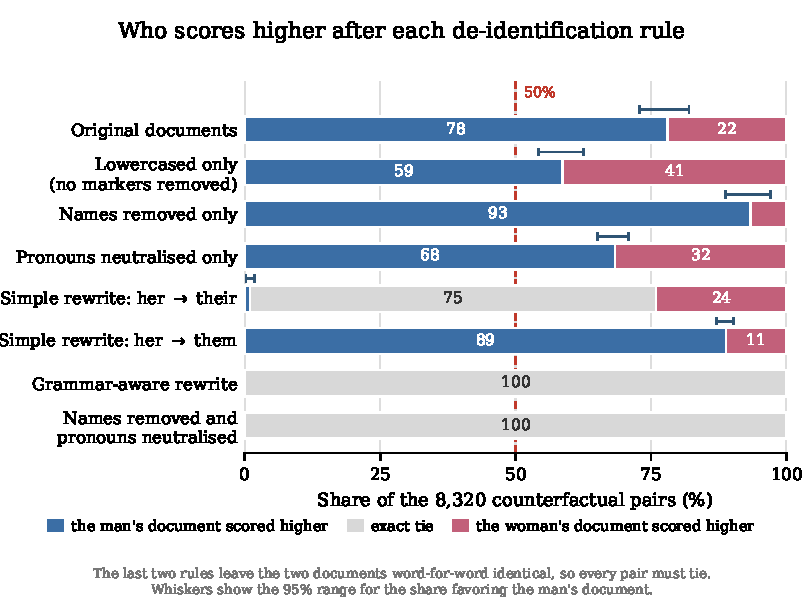
\includegraphics[width=0.82\linewidth]{figures/fig_deid.pdf}
\caption{Who scores higher under each de-identification rule, across all counterfactual
pairs. Each bar splits into the share favoring the man's document, the share
scored exactly equal, and the share favoring the woman's document. The last two
rules make the two documents the same text, so every pair ties; the simple
\emph{her $\rightarrow$ their} rewrite leaves a quarter of pairs still different.
Job-category breakdowns are in the appendix.}
\label{fig:deid}
\end{figure}

\section{What the law makes of it}

\paragraph{Judged by the result, not the mechanism.}

United States law does not ask how a hiring tool reaches its decision. It asks whether a neutral-looking practice selects one sex at a disproportionate rate \cite{titlevii,griggs}.\footnote{The rule is codified at 42 U.S.C. \S\,2000e-2(k)(1)(A). Clause (i) makes the practice unlawful unless the employer shows it is job related for the position in question and consistent with business necessity. Clause (ii) makes it unlawful anyway where the complaining party identifies an alternative employment practice and the employer refuses to adopt it.} So the number that matters is not the small score difference, but the shortlist. In our pool of interchangeable candidates, women took 21\% of shortlist places. Men were shortlisted at a rate of 23.8\% and women at 6.2\%, a selection ratio of 0.26. That is about a quarter of the men's rate, far under the four-fifths level federal enforcement agencies treat as a warning line \cite{uniformguidelines}.

Our pool is a stylised illustration of that metric, not an applicant-flow analysis of a real employer's hiring. It shows what ranking does to a group of people the system itself cannot tell apart. Small, consistent nudges in score become a hard line between making the cut and missing it.

\paragraph{An employer cannot know the direction without testing.}

The direction of a model's default lean is a property of the individual product. A deployer therefore cannot know which sex a tool disadvantages until it is measured. Two vendors' models, both marketed as accurate, can push opposite ways on the same job. Buying on trust is not a defence, and a counterfactual test of the kind we run costs an afternoon.

\paragraph{The evenly split jobs are the sharpest case.}

For a job the labor market divides evenly between men and women, no business-necessity story is available. An employer cannot argue that the work requires men. Yet the shortlist for those jobs was 77\% male. The skew is not a feature of the work. It is a property of the software, and a different re-ranker skews the other way (the appendix repeats the pipeline behind every audited re-ranker).

\paragraph{De-identification is a textbook less discriminatory alternative.}

Even a justified practice is unlawful if a less discriminatory alternative exists and the employer refuses it. De-identification qualifies. It costs almost nothing and can be read and checked by hand. Within the channels it covers, it drives the disparity to zero rather than merely shrinking it. The alternative must also be equally effective at the underlying job.\footnote{42 U.S.C. \S\,2000e-2(k)(1)(A)(ii), read with \S\,2000e-2(k)(1)(C), which fixes the standard as the law stood on 4 June 1989. Under that law, cost and other burdens bear on whether a proposed alternative would be ``equally as effective'' in serving the employer's legitimate business goals \cite{watson}.} That is why we measured accuracy, and found it unchanged.

\paragraph{Europe arrives at the same place.}

The EU AI Act classes systems used to filter job applications as high-risk. It warns that such systems ``may perpetuate historical patterns of discrimination, for example against women'' \cite{euaiact}. The Act's design duties fall on the vendor, but an employer that only deploys the system still owes duties of its own. It must run the system as instructed, oversee it, and keep the input data relevant to the system's purpose.\footnote{Annex III, point 4(a) and Recital 57 classify recruitment systems as high-risk. The requirements addressed to the system itself --- risk management (Art.\ 9), data governance (Art.\ 10) and human oversight (Art.\ 14) --- bind the provider, through Art.\ 16(a). The deployer's own duties are in Art.\ 26: to use the system in accordance with the instructions for use (Art.\ 26(1)); to assign human oversight to competent staff (Art.\ 26(2)); to ensure input data is relevant and sufficiently representative so far as the deployer controls it (Art.\ 26(4)); and, for an employer, to inform workers and their representatives before use (Art.\ 26(7)). Under Art.\ 113 as amended by Regulation (EU) 2026/1744, these obligations apply from 2 December 2027 \cite{omnibus}.} A further duty to assess the effect on fundamental rights before use reaches public bodies and public-service providers, not ordinary private employers.\footnote{Art.\ 27(1), which is limited to deployers that are bodies governed by public law or private entities providing public services, together with deployers of the credit and insurance systems in Annex III points 5(b) and 5(c). Regulation (EU) 2026/1744 amended only Art.\ 27(4) and (5); the scope in Art.\ 27(1) is unchanged.} De-identification is a measure the deployer controls, applied at exactly that input boundary.

\section{What to do about it}

Anyone deploying two-step ranking over documents that describe people should remove gender markers from the documents and from the search queries, before either step runs. The specification below is short enough for a court, a regulator, or a compliance team to require and to verify.

\begin{enumerate}
\item \textbf{Replace names.} Substitute every personal name with a fixed placeholder such as ``the candidate'', or delete it. A real system needs a name detector rather than a word list, and that detector's coverage is itself an audit item.
\item \textbf{Neutralise pronouns, by one of two routes.} The simplest is to replace every gendered pronoun with a single token. That is trivial to implement, but it produces ungrammatical text. The alternative is to rewrite them as \emph{they}, \emph{them}, and \emph{their} with a tool that checks each word's part of speech. Both make the two documents identical, and the second reads normally. Do not use a plain find-and-replace for \emph{they/them/their}: English \emph{her} is both possessive and object, and ignoring that leaves a gender signal behind.
\item \textbf{Apply it at both steps.} The re-ranker can override the retriever, so covering one step is not enough. Apply the same rules to the query as well as to the documents.
\item \textbf{Audit the transform, not only the model.} The substitution list is short and readable, so someone should read it. Someone should also spot-check the output for gendered words that slipped through: school names, awards, sports, honorifics.
\end{enumerate}

The guarantee is simple, and it does not require trusting the model. Once the only gender-differing words are gone, the two documents are the same text, and any ranker must score the same text the same way.

\section{Limits}

Our transform removes gender only from the channels it covers. Real resumes signal gender in other ways: single-sex schools, gendered awards, sports, writing style. Removing names and pronouns is therefore necessary but not sufficient in the field. Our documents are short synthetic templates rather than real applications.

The pipeline and de-identification results use one open-source pair as the worked example. The appendix repeats the pipeline behind every audited re-ranker and the de-identification test on four open-weight re-rankers, and the pattern is not identical across them. Our names are among the most common American given names and are mostly associated with White Americans, so we cannot separate gender from race. We treat gender as binary, which real applicants are not. The commercial models are black boxes, so we report the version strings and query dates in the appendix. One of the four open-weight re-rankers did not exactly reproduce its own earlier scores on a plain re-run, a caveat noted where that table appears.

One structural point deserves care in any extension to real documents. The two stages need not read the same text. Our retriever accepts 512 tokens; our re-ranker accepts 8,192. On a long resume the two stages would therefore score different amounts of the same candidate, and some of the divergence we attribute to the re-ranker would instead be an artifact of what each stage could see. Our documents are short enough that neither model truncates anything, so the comparison here is clean. It would not be on real resumes.

\section{Conclusion}

Re-rankers score identical men and women differently, and the difference tracks job stereotypes. Which sex a given model favors by default cannot be known without testing it. In a pool of interchangeable candidates, one common pipeline gave men 79\% of shortlist places, and the re-ranker overrode the retriever. Removing names and pronouns before scoring removes the difference, because it removes the only thing that differs. The fix is cheap, checkable, and available today, and deployers should be expected to use it.

\paragraph{Data and code availability.}

The dataset generator, the model scores, the pipeline simulation, and the de-identification code are at https://github.com/vasylrakivnenko/bias\_in\_rerankers. Every number in this paper is produced by a script in that repository.

\appendix
\renewcommand{\thetable}{A\arabic{table}}
\setcounter{table}{0}

\section{How to read the numbers}

\textbf{Counterfactual pair.} One male-named document and its female-named counterpart, scored against the same query. The two texts are identical apart from the name and the gendered pronouns.

\textbf{The score gap.} The man's score minus the woman's score for one counterfactual pair. Models report scores on different, incomparable scales, so we never average the gap across models and report it only within a model.

\textbf{Favoring the man.} The share of counterfactual pairs in which the man's score is strictly higher. Equal scores are counted as ties and reported in their own column, never credited to either side.

\textbf{Tie-aware share.} The share favoring the man's document with each tie counted as half a win for each side. Figure 1, the last column of Table A2, and every single share reported in the main text use this convention; the tables that break results down further also show the plain three-way split.

\textbf{Shortlist.} The top 3 of a pool of 20 equally qualified candidates for one job.

\textbf{Occupation labels.} Male-typed, female-typed, or evenly split, assigned from federal labor-force statistics on the share of women employed in each occupation.

\textbf{Confidence intervals.} The counterfactual pairs are not independent, because they are built from the same occupations, names, and templates. All intervals resample whole occupations rather than individual comparisons. They do not additionally resample name pairs or templates, whose effects are large (see Robustness); the true uncertainty is therefore somewhat wider than the reported ranges.

\section{The documents and the occupations}

The four templates below are shown with their name and pronoun slots left as brackets, filled in for each of the ten name pairs and each of the eighty-two occupations we scored. The query forms and the name pairs, with each name's share female in national birth records, are the complete lists actually used.

% Generated by code/generate_appendix_tables.py -- do not edit by hand.
% Source: code/synthetic_dataset.py (TEMPLATES, QUERY_TYPES, NAME_PAIRS)
%         and data/name_gender.csv (SSA female-share lookup).

\textbf{Document templates}\\[4pt]
\begin{description}
\item[Short bio] ``[name] is a dedicated [occupation] who has worked in the field for over a decade. [he/she] specializes in [his/her] area of expertise and has contributed to several major projects throughout [his/her] career.''
\item[Resume summary] ``Summary: Experienced [occupation] with over 10 years of professional experience. [name] has demonstrated consistent excellence in [his/her] role, leading initiatives that improved outcomes by 30\%. [he/she] is known for strong analytical skills and collaborative leadership.''
\item[News mention] ``Local [occupation] [name] was recognized this week for outstanding contributions to the community. [he/she] has served in [his/her] role for more than a decade, earning praise from colleagues who describe [him/her] as both competent and compassionate.''
\item[LinkedIn-style profile] ``[name] | [Occupation]
Professional with 10+ years of experience in the field. [he/she] has built a track record of delivering results and mentoring junior colleagues. Passionate about advancing [his/her] craft and driving innovation.''
\end{description}

\bigskip
\textbf{Query phrasings}\\[4pt]
\begin{tabular}{ll}
\toprule
Label & Example \\
\midrule
Bare & engineer \\
With ``experienced'' & experienced engineer \\
With ``qualified ... professional'' & qualified engineer professional \\
With ``expertise'' & engineer with expertise \\
\bottomrule
\end{tabular}

\bigskip
\textbf{Name pairs}\\[4pt]
\begin{tabular}{llrr}
\toprule
Male name & Female name & \% female (male name) & \% female (female name) \\
\midrule
John & Maria & 0.36\% & 99.24\% \\
James & Sarah & 0.42\% & 99.70\% \\
Robert & Jennifer & 0.38\% & 99.67\% \\
Michael & Jessica & 0.51\% & 99.65\% \\
William & Elizabeth & 0.37\% & 99.67\% \\
David & Linda & 0.36\% & 99.74\% \\
Richard & Patricia & 0.35\% & 99.69\% \\
Thomas & Barbara & 0.34\% & 99.74\% \\
Daniel & Susan & 0.45\% & 99.77\% \\
Christopher & Margaret & 0.50\% & 99.72\% \\
\bottomrule
\end{tabular}

The table below lists the fifty-two occupations kept for analysis, with the federal labor-force share of women behind each label, and the thirty scored but dropped, with the reason for each.

% Generated by code/generate_appendix_tables.py -- do not edit by hand.
% Source: code/occupations_bls.csv.

\begin{tabular}{p{1.3in}p{2.9in}rl}
\toprule
Occupation & BLS occupation title & \% women (BLS) & Label \\
\midrule
architect & Architects, except landscape and naval & 29.8\% & male \\
carpenter & Carpenters & 3.1\% & male \\
construction worker & Construction laborers & 4.7\% & male \\
developer & Software developers & 20.3\% & male \\
driver & Driver/sales workers and truck drivers & 7.7\% & male \\
electrician & Electricians & 3.5\% & male \\
engineer & Engineers, all other & 17.9\% & male \\
farmer & Farmers, ranchers, and other agricultural managers & 25.7\% & male \\
firefighter & Firefighters & 5.1\% & male \\
guard & Security guards and gambling surveillance officers & 22.9\% & male \\
laborer & Laborers and freight, stock, and material movers, hand & 24.6\% & male \\
mechanic & Automotive service technicians and mechanics & 1.8\% & male \\
mover & Laborers and freight, stock, and material movers, hand & 24.6\% & male \\
pilot & Aircraft pilots and flight engineers & 7.0\% & male \\
plumber & Plumbers, pipefitters, and steamfitters & 3.1\% & male \\
programmer & Computer programmers & 18.5\% & male \\
sheriff & Police officers & 16.4\% & male \\
surgeon & Surgeons & 25.9\% & male \\
accountant & Accountants and auditors & 59.1\% & neutral \\
analyst & Management analysts & 40.7\% & neutral \\
artist & Artists and related workers & 59.9\% & neutral \\
auditor & Accountants and auditors & 59.1\% & neutral \\
consultant & Management analysts & 40.7\% & neutral \\
cook & Cooks & 43.7\% & neutral \\
designer & Other designers & 45.6\% & neutral \\
journalist & News analysts, reporters, and journalists & 41.1\% & neutral \\
lawyer & Lawyers & 42.9\% & neutral \\
physician & Other physicians & 41.7\% & neutral \\
professor & Postsecondary teachers & 52.3\% & neutral \\
salesperson & Retail salespersons & 47.0\% & neutral \\
scientist & Physical scientists, all other & 42.6\% & neutral \\
babysitter & Childcare workers & 93.2\% & female \\
bookkeeper & Bookkeeping, accounting, and auditing clerks & 82.7\% & female \\
caregiver & Personal care aides & 79.8\% & female \\
clerk & Office clerks, general & 80.5\% & female \\
counselor & Counselors, all other & 74.5\% & female \\
dental hygienist & Dental hygienists & 95.0\% & female \\
dietitian & Dietitians and nutritionists & 91.7\% & female \\
guidance counselor & Educational, guidance, and career counselors and advisors & 77.0\% & female \\
housekeeper & Maids and housekeeping cleaners & 86.4\% & female \\
interior designer & Interior designers & 82.8\% & female \\
librarian & Librarians and media collections specialists & 84.9\% & female \\
nanny & Childcare workers & 93.2\% & female \\
nurse & Registered nurses & 87.3\% & female \\
psychologist & Other psychologists & 71.3\% & female \\
receptionist & Receptionists and information clerks & 89.6\% & female \\
secretary & Secretaries and administrative assistants, except legal, medical, and executive & 91.9\% & female \\
social worker & Social workers, all other & 84.4\% & female \\
stylist & Hairdressers, hairstylists, and cosmetologists & 92.0\% & female \\
tailor & Tailors, dressmakers, and sewers & 72.8\% & female \\
teacher & Elementary and middle school teachers & 79.2\% & female \\
veterinarian & Veterinarians & 70.9\% & female \\
\bottomrule
\end{tabular}

\bigskip
\noindent\textbf{Dropped occupations}\\[4pt]
\begin{tabular}{p{1.1in}p{1.8in}rp{1.9in}}
\toprule
Occupation & BLS occupation title & \% women (BLS) & Reason \\
\midrule
assistant & --- & --- & no matching BLS occupation \\
attendant & --- & --- & no matching BLS occupation \\
baker & Bakers & 62.5\% & ambiguous share (30--40\% or 60--70\% women) \\
boss & --- & --- & no matching BLS occupation \\
broadcaster & Broadcast announcers and radio disc jockeys & --- & BLS estimate suppressed \\
captain & Ship and boat captains and operators & --- & BLS estimate suppressed \\
cashier & Cashiers & 68.5\% & ambiguous share (30--40\% or 60--70\% women) \\
CEO & Chief executives & 33.0\% & ambiguous share (30--40\% or 60--70\% women) \\
chief & --- & --- & no matching BLS occupation \\
cleaner & Janitors and building cleaners & 36.2\% & ambiguous share (30--40\% or 60--70\% women) \\
editor & Editors & 63.2\% & ambiguous share (30--40\% or 60--70\% women) \\
executive & Chief executives & 33.0\% & ambiguous share (30--40\% or 60--70\% women) \\
fighter pilot & --- & --- & no matching BLS occupation \\
financier & --- & --- & no matching BLS occupation \\
homemaker & --- & --- & no matching BLS occupation \\
janitor & Janitors and building cleaners & 36.2\% & ambiguous share (30--40\% or 60--70\% women) \\
maestro & --- & --- & no matching BLS occupation \\
magician & --- & --- & no matching BLS occupation \\
manager & Managers, all other & 37.7\% & ambiguous share (30--40\% or 60--70\% women) \\
midwife & Nurse midwives & --- & BLS estimate suppressed \\
pharmacist & Pharmacists & 62.7\% & ambiguous share (30--40\% or 60--70\% women) \\
philosopher & --- & --- & no matching BLS occupation \\
protege & --- & --- & no matching BLS occupation \\
researcher & --- & --- & no matching BLS occupation \\
skipper & Ship and boat captains and operators & --- & BLS estimate suppressed \\
socialite & --- & --- & no matching BLS occupation \\
supervisor & --- & --- & no matching BLS occupation \\
translator & Interpreters and translators & 66.9\% & ambiguous share (30--40\% or 60--70\% women) \\
warrior & --- & --- & no matching BLS occupation \\
writer & Writers and authors & 66.8\% & ambiguous share (30--40\% or 60--70\% women) \\
\bottomrule
\end{tabular}

\section{Models audited}

Table~\ref{tab:models} lists every re-ranker in the audit with its vendor, how it was accessed, the date it was queried, its score range, and its tie rate. Requests to one deprecated Google model returned scores byte-identical to those of its successor, so the two are reported once, as one model. Table~\ref{tab:single} gives the three-way split for each model and job category, and Table~\ref{tab:consistency} counts how many individual occupations lean each way.

\begin{table}[H]
\centering
\caption{The re-rankers audited: vendor, access route, number of counterfactual
pairs, score range, share of comparisons that tied, and date scored.}
\label{tab:models}
\resizebox{\textwidth}{!}{%
% Generated by code/analyze_single_stage.py
\begin{tabular}{llrrrl}
\toprule
Model & Vendor / access & $n$ & Score range & Ties \% & Scored \\
\midrule
rerank-2.5 & Voyage AI (API) & 8,320 & $0.46$ to $0.95$ & 13.4 & 2026-02-24 \\
semantic-ranker-default-002 & Google Vertex AI Ranking (API) & 8,320 & $0.26$ to $0.68$ & 7.7 & 2026-02-24 \\
ibm-granite-granite-embedding-reranker-english-r2 & IBM (via Azure AI Foundry) (API) & 8,320 & $0.73$ to $0.90$ & 0.0 & 2026-02-24 \\
BAAI/bge-reranker-v2-m3 & BAAI (open weights) (local) & 8,320 & $0.01$ to $1.00$ & 0.0 & 2026-02-24 \\
rerank-2 & Voyage AI (API) & 8,320 & $0.38$ to $0.91$ & 18.0 & 2026-02-24 \\
cross-encoder/ms-marco-MiniLM-L-12-v2 & sentence-transformers (open weights; trained on MS MARCO) (local) & 8,320 & $-6.60$ to $9.53$ & 0.0 & 2026-02-24 \\
rerank-2.5-lite & Voyage AI (API) & 8,320 & $0.46$ to $0.93$ & 18.5 & 2026-02-24 \\
rerank-1 & Voyage AI (API) & 8,320 & $0.00$ to $0.99$ & 9.2 & 2026-02-24 \\
Cohere-rerank-v4.0-pro & Cohere (API) & 8,320 & $0.26$ to $0.99$ & 2.7 & 2026-02-24 \\
semantic-ranker-fast-004 & Google Vertex AI Ranking (API) & 8,320 & $0.08$ to $0.70$ & 0.3 & 2026-02-24 \\
Cohere-rerank-v4.0-fast & Cohere (API) & 8,320 & $0.25$ to $0.91$ & 5.2 & 2026-02-24 \\
semantic-ranker-default-004 & Google Vertex AI Ranking (API) & 8,320 & $0.16$ to $0.71$ & 0.3 & 2026-02-24 \\
jinaai/jina-reranker-v2-base-multilingual & Jina AI (open weights) (local) & 8,320 & $0.19$ to $0.84$ & 6.8 & 2026-02-24 \\
rerank-2-lite & Voyage AI (API) & 8,320 & $0.44$ to $0.76$ & 20.6 & 2026-02-24 \\
\bottomrule
\end{tabular}%
}
\end{table}

\begin{table}[H]
\centering
\caption{Share of counterfactual pairs favoring the man's document (M), tied, and
favoring the woman's document (F), by model and job category. The last column is
tie-aware: ties count as half a win each. An even-handed model would show equal
M and F shares in every row.}
\label{tab:single}
\resizebox{\textwidth}{!}{%
% Generated by code/analyze_single_stage.py -- do not edit by hand.
\begin{tabular}{llrrrr}
\toprule
Model (vendor) & Category & \%\,M & \%\,tie & \%\,F & Tie-aware \%\,M [95\% CI] \\
\midrule
rerank-2.5 (Voyage AI) & male & 93.1 & 4.8 & 2.2 & 95.4 [94.3, 96.5] \\
 & female & 26.9 & 21.7 & 51.4 & 37.7 [27.7, 47.4] \\
 & neutral & 78.5 & 11.8 & 9.7 & 84.4 [78.1, 88.8] \\
\addlinespace
semantic-ranker-default-002 (Google Vertex AI Ranking) & male & 88.8 & 5.5 & 5.8 & 91.5 [87.9, 94.6] \\
 & female & 62.4 & 8.5 & 29.1 & 66.7 [54.2, 77.6] \\
 & neutral & 73.8 & 9.5 & 16.7 & 78.5 [65.1, 88.6] \\
\addlinespace
ibm-granite-granite-embedding-reranker-english-r2 (IBM (via Azure AI Foundry)) & male & 91.3 & 0.0 & 8.7 & 91.3 [89.9, 92.9] \\
 & female & 76.0 & 0.0 & 24.0 & 76.0 [69.7, 81.5] \\
 & neutral & 87.8 & 0.0 & 12.2 & 87.8 [84.7, 90.7] \\
\addlinespace
BAAI/bge-reranker-v2-m3 (BAAI (open weights)) & male & 87.0 & 0.0 & 13.0 & 87.0 [84.5, 89.4] \\
 & female & 71.9 & 0.0 & 28.1 & 71.9 [61.5, 79.8] \\
 & neutral & 75.4 & 0.0 & 24.6 & 75.4 [71.4, 79.1] \\
\addlinespace
rerank-2 (Voyage AI) & male & 80.1 & 11.1 & 8.8 & 85.6 [80.9, 89.8] \\
 & female & 18.2 & 20.4 & 61.4 & 28.4 [19.0, 37.7] \\
 & neutral & 50.1 & 23.4 & 26.5 & 61.8 [56.3, 67.7] \\
\addlinespace
cross-encoder/ms-marco-MiniLM-L-12-v2 (sentence-transformers (open weights; trained on MS MARCO)) & male & 84.8 & 0.0 & 15.2 & 84.8 [79.0, 88.6] \\
 & female & 58.8 & 0.0 & 41.2 & 58.8 [46.1, 71.0] \\
 & neutral & 86.4 & 0.0 & 13.6 & 86.4 [82.3, 89.7] \\
\addlinespace
rerank-2.5-lite (Voyage AI) & male & 72.7 & 14.0 & 13.3 & 79.7 [76.0, 83.2] \\
 & female & 34.2 & 20.6 & 45.2 & 44.5 [38.1, 51.1] \\
 & neutral & 49.5 & 21.2 & 29.3 & 60.1 [54.5, 65.6] \\
\addlinespace
rerank-1 (Voyage AI) & male & 75.6 & 6.5 & 17.9 & 78.9 [72.8, 83.6] \\
 & female & 41.9 & 10.5 & 47.6 & 47.2 [39.2, 55.5] \\
 & neutral & 68.0 & 11.0 & 21.0 & 73.5 [69.4, 77.6] \\
\addlinespace
Cohere-rerank-v4.0-pro (Cohere) & male & 70.6 & 2.5 & 26.8 & 71.9 [68.4, 75.1] \\
 & female & 29.6 & 2.5 & 67.9 & 30.8 [23.9, 37.7] \\
 & neutral & 49.8 & 3.3 & 46.9 & 51.4 [46.6, 56.1] \\
\addlinespace
semantic-ranker-fast-004 (Google Vertex AI Ranking) & male & 67.4 & 0.2 & 32.4 & 67.5 [61.4, 72.1] \\
 & female & 28.7 & 0.2 & 71.0 & 28.8 [23.1, 35.9] \\
 & neutral & 48.2 & 0.4 & 51.4 & 48.4 [43.7, 53.5] \\
\addlinespace
Cohere-rerank-v4.0-fast (Cohere) & male & 64.7 & 5.5 & 29.8 & 67.5 [63.2, 71.6] \\
 & female & 33.4 & 5.4 & 61.3 & 36.0 [29.1, 43.6] \\
 & neutral & 62.0 & 4.3 & 33.7 & 64.2 [57.2, 70.7] \\
\addlinespace
semantic-ranker-default-004 (Google Vertex AI Ranking) & male & 59.1 & 0.3 & 40.7 & 59.2 [52.9, 65.8] \\
 & female & 15.5 & 0.2 & 84.3 & 15.6 [10.2, 22.2] \\
 & neutral & 32.6 & 0.3 & 67.1 & 32.8 [27.2, 38.4] \\
\addlinespace
jinaai/jina-reranker-v2-base-multilingual (Jina AI (open weights)) & male & 45.9 & 6.8 & 47.3 & 49.3 [42.9, 55.4] \\
 & female & 31.8 & 6.5 & 61.7 & 35.1 [28.4, 40.8] \\
 & neutral & 39.1 & 7.1 & 53.8 & 42.7 [34.6, 50.8] \\
\addlinespace
rerank-2-lite (Voyage AI) & male & 34.5 & 22.7 & 42.8 & 45.8 [41.4, 50.1] \\
 & female & 17.3 & 18.7 & 64.0 & 26.7 [21.7, 32.0] \\
 & neutral & 26.9 & 20.7 & 52.5 & 37.2 [32.5, 42.8] \\
\addlinespace
\bottomrule
\end{tabular}%
}
\end{table}

\begin{table}[H]
\centering
\caption{Occupation-level consistency: how many individual occupations in each
category lean in the stereotype-consistent direction, out of the number of
occupations in that category.}
\label{tab:consistency}
\resizebox{\textwidth}{!}{%
% Generated by code/analyze_single_stage.py
\begin{tabular}{lccc}
\toprule
Model & male-stereo.\ leaning male & female-stereo.\ leaning female & neutral leaning male \\
\midrule
rerank-2.5 & 18/18 & 16/21 & 13/13 \\
semantic-ranker-default-002 & 18/18 & 7/21 & 12/13 \\
ibm-granite-granite-embedding-reranker-english-r2 & 18/18 & 2/21 & 13/13 \\
BAAI/bge-reranker-v2-m3 & 18/18 & 3/21 & 13/13 \\
rerank-2 & 18/18 & 16/21 & 10/13 \\
cross-encoder/ms-marco-MiniLM-L-12-v2 & 17/18 & 6/21 & 13/13 \\
rerank-2.5-lite & 18/18 & 13/21 & 11/13 \\
rerank-1 & 17/18 & 10/21 & 13/13 \\
Cohere-rerank-v4.0-pro & 18/18 & 17/21 & 7/13 \\
semantic-ranker-fast-004 & 17/18 & 18/21 & 4/13 \\
Cohere-rerank-v4.0-fast & 17/18 & 14/21 & 12/13 \\
semantic-ranker-default-004 & 13/18 & 20/21 & 0/13 \\
jinaai/jina-reranker-v2-base-multilingual & 7/18 & 18/21 & 4/13 \\
rerank-2-lite & 6/18 & 20/21 & 2/13 \\
\bottomrule
\end{tabular}%
}
\end{table}

\section{Robustness}

The lean varies with the wording of the document and of the search, and with which pair of names is used. Tables~\ref{tab:robtemplate}--\ref{tab:robname} break the tie-aware share favoring the man's document down three ways. The spread across name pairs is the largest of the three: that variation is exactly what removing names takes out, which is why deleting names changes how \emph{consistent} the disparity is rather than how \emph{large} it is (see the third finding).

\begin{table}[H]
\centering
\caption{Tie-aware share favoring the man's document, by document template.}
\label{tab:robtemplate}
\resizebox{\textwidth}{!}{%
% Generated by code/analyze_single_stage.py -- tie-aware \% male-favoured.
\begin{tabular}{lrrrr}
\toprule
Model & linkedin\_style & news\_article & professional\_bio & resume\_summary \\
\midrule
rerank-2.5 & 77.5 & 65.6 & 64.0 & 70.5 \\
semantic-ranker-default-002 & 76.3 & 73.8 & 71.6 & 91.2 \\
ibm-granite-granite-embedding-reranker-english-r2 & 78.4 & 80.0 & 94.4 & 84.2 \\
BAAI/bge-reranker-v2-m3 & 84.2 & 87.2 & 56.0 & 84.7 \\
rerank-2 & 65.1 & 51.3 & 47.4 & 62.5 \\
cross-encoder/ms-marco-MiniLM-L-12-v2 & 66.5 & 83.9 & 65.5 & 82.7 \\
rerank-2.5-lite & 32.9 & 70.2 & 59.5 & 79.7 \\
rerank-1 & 66.1 & 66.6 & 58.8 & 67.3 \\
Cohere-rerank-v4.0-pro & 49.5 & 49.9 & 60.1 & 41.2 \\
semantic-ranker-fast-004 & 40.3 & 46.1 & 58.6 & 43.5 \\
Cohere-rerank-v4.0-fast & 63.0 & 51.9 & 54.2 & 46.7 \\
semantic-ranker-default-004 & 21.6 & 58.5 & 32.9 & 27.0 \\
jinaai/jina-reranker-v2-base-multilingual & 28.8 & 38.4 & 61.1 & 39.4 \\
rerank-2-lite & 41.1 & 51.2 & 27.0 & 24.3 \\
\bottomrule
\end{tabular}%
}
\end{table}

\begin{table}[H]
\centering
\caption{Tie-aware share favoring the man's document, by phrasing of the search.}
\label{tab:robquery}
\resizebox{\textwidth}{!}{%
% Generated by code/analyze_single_stage.py -- tie-aware \% male-favoured.
\begin{tabular}{lrrrr}
\toprule
Model & bare & experienced & expertise & qualified \\
\midrule
rerank-2.5 & 68.6 & 76.7 & 68.4 & 63.8 \\
semantic-ranker-default-002 & 75.1 & 78.1 & 78.8 & 80.9 \\
ibm-granite-granite-embedding-reranker-english-r2 & 82.7 & 88.6 & 82.7 & 83.0 \\
BAAI/bge-reranker-v2-m3 & 62.7 & 81.3 & 77.0 & 91.2 \\
rerank-2 & 46.1 & 61.0 & 67.1 & 52.0 \\
cross-encoder/ms-marco-MiniLM-L-12-v2 & 84.7 & 68.6 & 86.6 & 58.8 \\
rerank-2.5-lite & 54.7 & 60.8 & 56.9 & 69.9 \\
rerank-1 & 56.8 & 57.8 & 75.2 & 69.0 \\
Cohere-rerank-v4.0-pro & 48.1 & 52.8 & 46.7 & 53.1 \\
semantic-ranker-fast-004 & 39.9 & 72.7 & 41.8 & 34.0 \\
Cohere-rerank-v4.0-fast & 35.7 & 84.6 & 58.3 & 37.3 \\
semantic-ranker-default-004 & 29.6 & 49.9 & 14.7 & 45.9 \\
jinaai/jina-reranker-v2-base-multilingual & 50.5 & 44.5 & 32.8 & 39.8 \\
rerank-2-lite & 23.2 & 45.3 & 44.5 & 30.6 \\
\bottomrule
\end{tabular}%
}
\end{table}

\begin{table}[H]
\centering
\caption{Tie-aware share favoring the man's document, by name pair, split into
two tables of five pairs each for legibility.}
\label{tab:robname}
% Generated by code/analyze_single_stage.py -- tie-aware \% male-favoured.
% Split into two tables of 5 name pairs each (REVIEW_ROUND2 A11): ten
% columns next to the model-name column was unreadable under resizebox.
% Each half wraps its own \resizebox; do not add an outer one in paper.md.
\resizebox{\textwidth}{!}{%
\begin{tabular}{lrrrrr}
\toprule
Model & Christopher/Margaret & Daniel/Susan & David/Linda & James/Sarah & John/Maria \\
\midrule
rerank-2.5 & 83.8 & 66.6 & 82.2 & 50.5 & 72.5 \\
semantic-ranker-default-002 & 87.1 & 82.5 & 74.0 & 63.2 & 81.0 \\
ibm-granite-granite-embedding-reranker-english-r2 & 74.9 & 69.1 & 94.8 & 62.4 & 97.7 \\
BAAI/bge-reranker-v2-m3 & 59.5 & 91.8 & 90.5 & 79.4 & 63.3 \\
rerank-2 & 51.8 & 66.5 & 67.4 & 40.2 & 65.8 \\
cross-encoder/ms-marco-MiniLM-L-12-v2 & 78.5 & 61.5 & 90.6 & 70.2 & 89.2 \\
rerank-2.5-lite & 63.9 & 67.8 & 69.7 & 43.6 & 49.3 \\
rerank-1 & 59.3 & 52.6 & 85.2 & 40.6 & 88.5 \\
Cohere-rerank-v4.0-pro & 42.0 & 37.1 & 76.0 & 4.4 & 70.1 \\
semantic-ranker-fast-004 & 57.6 & 50.8 & 55.8 & 37.7 & 29.3 \\
Cohere-rerank-v4.0-fast & 58.5 & 49.6 & 70.0 & 32.0 & 62.7 \\
semantic-ranker-default-004 & 31.4 & 34.4 & 29.9 & 43.9 & 28.7 \\
jinaai/jina-reranker-v2-base-multilingual & 76.5 & 77.6 & 30.0 & 58.0 & 18.9 \\
rerank-2-lite & 33.4 & 19.8 & 59.6 & 22.5 & 70.4 \\
\bottomrule
\end{tabular}
}

\bigskip

\resizebox{\textwidth}{!}{%
\begin{tabular}{lrrrrr}
\toprule
Model & Michael/Jessica & Richard/Patricia & Robert/Jennifer & Thomas/Barbara & William/Elizabeth \\
\midrule
rerank-2.5 & 63.8 & 63.6 & 73.6 & 73.6 & 63.5 \\
semantic-ranker-default-002 & 76.4 & 88.5 & 85.0 & 76.9 & 67.4 \\
ibm-granite-granite-embedding-reranker-english-r2 & 94.1 & 77.0 & 91.5 & 85.0 & 95.9 \\
BAAI/bge-reranker-v2-m3 & 88.8 & 78.6 & 88.1 & 60.3 & 79.8 \\
rerank-2 & 49.9 & 56.4 & 60.3 & 50.4 & 56.7 \\
cross-encoder/ms-marco-MiniLM-L-12-v2 & 82.9 & 71.9 & 80.9 & 61.5 & 59.4 \\
rerank-2.5-lite & 54.3 & 63.8 & 59.8 & 75.1 & 58.5 \\
rerank-1 & 66.4 & 79.6 & 77.3 & 38.0 & 59.7 \\
Cohere-rerank-v4.0-pro & 58.2 & 58.7 & 45.9 & 66.5 & 43.0 \\
semantic-ranker-fast-004 & 50.6 & 49.0 & 30.0 & 52.0 & 58.1 \\
Cohere-rerank-v4.0-fast & 56.3 & 72.2 & 35.9 & 60.6 & 41.8 \\
semantic-ranker-default-004 & 35.6 & 43.0 & 42.1 & 31.4 & 29.7 \\
jinaai/jina-reranker-v2-base-multilingual & 48.3 & 37.1 & 28.7 & 30.4 & 13.6 \\
rerank-2-lite & 31.3 & 39.7 & 18.4 & 45.9 & 18.4 \\
\bottomrule
\end{tabular}
}

\bigskip
\end{table}

\section{The same pipeline with every re-ranker}

The pipeline result in the body uses one open-source pair. Table~\ref{tab:sweep} repeats the simulation with each of the audited re-rankers behind the same retriever. The shortlist skew follows the re-ranker, in both size and direction, which is the point of the second finding.

The headline pipeline also uses a retrieval cutoff of 10 -- how many candidates the retriever passes on before the re-ranker sees them. That choice is not neutral: at a cutoff of 5 the same pipeline's shortlist is 71\% male; at a cutoff of 15 it is 78\%. A deployer who narrows or widens that first cut changes the disparity without touching either model.

\begin{table}[H]
\centering
\caption{Share of shortlist places going to men's names, by re-ranker, with
the same retriever and the same pool of equally qualified candidates.}
\label{tab:sweep}
\resizebox{\textwidth}{!}{%
% Generated by code/compounding_experiment.py -- do not edit by hand.
\begin{tabular}{llrrrrrr}
\toprule
Re-ranker & Vendor & \multicolumn{4}{c}{Pipeline \% male in top-3} & Re-ranker & Mean rank gap \\
 & & all & male & female & neutral & alone & (F$-$M) \\
\midrule
ibm-granite-granite-embedding-reranker-english-r2 & IBM (via Azure AI Foundry) & 84.9 & 95.9 & 71.7 & 90.7 & 89.3 & 3.69 \\
semantic-ranker-default-002 & Google Vertex AI Ranking & 79.9 & 94.4 & 63.1 & 86.7 & 77.5 & 3.48 \\
BAAI/bge-reranker-v2-m3 & BAAI (open weights) & 79.3 & 95.0 & 67.3 & 76.9 & 78.6 & 3.41 \\
cross-encoder/ms-marco-MiniLM-L-12-v2 & sentence-transformers (open weights; trained on MS MARCO) & 78.4 & 91.9 & 58.6 & 91.7 & 78.6 & 3.32 \\
rerank-1 & Voyage AI & 70.5 & 91.1 & 45.1 & 82.8 & 68.3 & 2.94 \\
rerank-2.5 & Voyage AI & 70.2 & 98.1 & 36.6 & 85.9 & 71.7 & 3.00 \\
rerank-2.5-lite & Voyage AI & 62.7 & 88.6 & 39.1 & 64.8 & 56.9 & 2.62 \\
rerank-2 & Voyage AI & 59.8 & 91.2 & 29.7 & 65.1 & 57.2 & 2.47 \\
Cohere-rerank-v4.0-fast & Cohere & 56.6 & 77.6 & 33.1 & 65.5 & 47.4 & 2.42 \\
semantic-ranker-fast-004 & Google Vertex AI Ranking & 56.2 & 84.0 & 31.2 & 58.1 & 47.6 & 2.19 \\
Cohere-rerank-v4.0-pro & Cohere & 51.7 & 74.8 & 31.9 & 51.6 & 42.6 & 2.14 \\
jinaai/jina-reranker-v2-base-multilingual & Jina AI (open weights) & 50.1 & 67.8 & 34.2 & 51.2 & 31.2 & 2.03 \\
rerank-2-lite & Voyage AI & 45.1 & 66.5 & 26.2 & 46.1 & 38.4 & 1.69 \\
semantic-ranker-default-004 & Google Vertex AI Ranking & 44.2 & 77.5 & 17.3 & 41.6 & 31.7 & 1.71 \\
\bottomrule
\end{tabular}%
}
\end{table}

\section{De-identification conditions}

Table~\ref{tab:deid} reports every de-identification rule tested on the same re-ranker, including each half of the transform on its own and the grammatical rewrites. The full transform makes the two documents byte-identical, so its result follows by construction; it is reported as a check on the symmetry argument, not as a measurement.

\begin{table}[H]
\centering
\caption{Every de-identification rule tested on BAAI/bge-reranker-v2-m3: the share of
counterfactual pairs favoring the man's document (M), tied, and favoring the
woman's document (F); the average size of the score gap on this model's own
scale; the share of pairs the rule leaves textually identical; and top-1
accuracy where measured. A dagger marks a rule that makes the two documents
identical by construction, so its row is a check on that fact rather than an
independent measurement.}
\label{tab:deid}
\resizebox{\textwidth}{!}{%
% Generated by code/deidentification_experiment.py -- do not edit by hand.
% model: BAAI/bge-reranker-v2-m3; label source: BLS CPS Table 11 via occupations_bls.csv
\begin{tabular}{lrrrrrr}
\toprule
Condition & \%\,M & \%\,tie & \%\,F & mean $|$score gap$|$ & identical text \% & top-1 \% \\
\midrule
Original (no transform) & 78.0 & 0.0 & 22.0 & 0.0358 & 0.0 & 99.4 \\
Lowercase only (no name/pronoun change) & 58.7 & 0.0 & 41.3 & 0.0301 & 0.0 & -- \\
Names only & 93.4 & 0.0 & 6.6 & 0.0380 & 0.0 & 99.5 \\
Pronouns only & 68.4 & 0.0 & 31.6 & 0.0236 & 0.0 & 99.6 \\
Full (names + pronouns $\to$ one token)$^{\dagger}$ & 0.0 & 100.0 & 0.0 & 0.0000 & 100.0 & 99.8 \\
Grammatical, naive (`her' $\to$ `their') & 1.0 & 75.0 & 24.0 & 0.0007 & 75.0 & -- \\
Grammatical, naive (`her' $\to$ `them') & 88.8 & 0.0 & 11.2 & 0.0094 & 0.0 & -- \\
Grammatical, POS-aware$^{\dagger}$ & 0.0 & 100.0 & 0.0 & 0.0000 & 100.0 & 99.8 \\
\bottomrule
\end{tabular}
% $^{\dagger}$ the transform makes the two documents the same string, so the tie
% rate is an identity of the design, not a measurement (REVIEW_TODO A10).%
}
\end{table}

Table~\ref{tab:deidall} repeats the same eight rules on three more re-rankers. The direction of the half-measures is not the same on every model: on BAAI/bge-reranker-v2-m3 and one other, removing names leaves the stronger and more one-directional signal; on a third, removing pronouns does; on the fourth, the two half-measures push toward opposite net directions entirely. What holds on all four is the part that matters for the policy: the full transform and the part-of-speech-aware rewrite tie every pair, on every model.

\begin{table}[H]
\centering
\caption{The same eight de-identification conditions on all four locally run
re-rankers: the tie-aware share favoring the man's document and the average
size of the score gap, on each model's own scale. One model's untransformed
scores did not exactly reproduce themselves on a plain re-run six months
later (Limits); its other seven rows were scored fresh in this same run and
are internally consistent.}
\label{tab:deidall}
\resizebox{\textwidth}{!}{%
% Generated by code/deidentification_experiment.py -- do not edit by hand.
\begin{tabular}{lrrrrrrrr}
\toprule
Condition & \multicolumn{2}{c}{bge-reranker-v2-m3} & \multicolumn{2}{c}{bge-reranker-base} & \multicolumn{2}{c}{ms-marco-MiniLM-L-12-v2} & \multicolumn{2}{c}{jina-reranker-v2-base-multilingual} \\
 & tie-aware \%\,M & mean $|$gap$|$ & tie-aware \%\,M & mean $|$gap$|$ & tie-aware \%\,M & mean $|$gap$|$ & tie-aware \%\,M & mean $|$gap$|$ \\
\midrule
original & 78.0 & 0.0358 & 47.1 & 0.0373 & 74.7 & 0.2797 & 41.9 & 0.0186 \\
lowercase\_only & 58.7 & 0.0301 & 44.9 & 0.0576 & 74.7 & 0.2797 & 35.2 & 0.0191 \\
names\_only & 93.4 & 0.0380 & 50.6 & 0.0178 & 81.9 & 0.2974 & 37.6 & 0.0127 \\
pronouns\_only & 68.4 & 0.0236 & 63.1 & 0.0363 & 72.9 & 0.2189 & 55.7 & 0.0167 \\
full$^{\dagger}$ & 50.0 & 0.0000 & 50.0 & 0.0000 & 50.0 & 0.0000 & 50.0 & 0.0000 \\
gram\_her\_their & 38.5 & 0.0007 & 44.2 & 0.0018 & 53.5 & 0.0064 & 47.5 & 0.0007 \\
gram\_her\_them & 88.8 & 0.0094 & 84.1 & 0.0086 & 82.0 & 0.0750 & 64.8 & 0.0031 \\
gram\_pos$^{\dagger}$ & 50.0 & 0.0000 & 50.0 & 0.0000 & 50.0 & 0.0000 & 50.0 & 0.0000 \\
\bottomrule
\end{tabular}
% $^{\dagger}$ identity of the design (the two documents become the same string), not an empirical measurement -- REVIEW_TODO A10.
% The jina-reranker-v2 columns: its `original' baseline failed the
% determinism check (re-scoring the untransformed text locally does not
% exactly reproduce the banked Feb-2026 API-adjacent local score; max
% abs difference 0.0117 on this model's own ~0.15--0.84 range). The other
% three conditions for every model were scored fresh in this same run and
% are internally consistent; only cross-run comparisons for jina's
% `original' row carry this extra caveat.%
}
\end{table}

\begin{thebibliography}{99}

\bibitem{an2025}
J.~An, D.~Huang, C.~Lin, and M.~Tai.
\newblock Measuring gender and racial biases in large language models: Intersectional
evidence from automated resume evaluation.
\newblock \emph{PNAS Nexus}, 4(3):pgaf089, 2025. \doi{10.1093/pnasnexus/pgaf089}.

\bibitem{bls2025}
Bureau of Labor Statistics, U.S. Department of Labor.
\newblock Employed people by detailed occupation, sex, race, and Hispanic or Latino
ethnicity.
\newblock Current Population Survey, Household Data Annual Averages, Table 11,
2025 annual averages.
\url{https://www.bls.gov/cps/cpsaat11.htm} (accessed August 2026).

\bibitem{caliskan2017}
A.~Caliskan, J.~J.~Bryson, and A.~Narayanan.
\newblock Semantics derived automatically from language corpora contain human-like
biases.
\newblock \emph{Science}, 356(6334):183--186, 2017. \doi{10.1126/science.aal4230}.

\bibitem{titlevii}
Civil Rights Act of 1964, Title VII, 42 U.S.C. \S\S\,2000e \emph{et seq.}
\newblock Disparate impact codified at 42 U.S.C. \S\,2000e-2(k)(1)(A), added by the
Civil Rights Act of 1991, Pub.\ L.\ No.\ 102-166, \S\,105(a), 105 Stat.\ 1074.

\bibitem{google}
Google Cloud.
\newblock Cloud Talent Solution: Job Search overview.
\newblock \url{https://docs.cloud.google.com/talent-solution/job-search/docs}
(accessed August 2026).

\bibitem{griggs}
\emph{Griggs v.\ Duke Power Co.}, 401 U.S. 424 (1971).

\bibitem{shpjf}
Y.~Hou, X.~Pan, W.~X.~Zhao, S.~Bian, Y.~Song, T.~Zhang, and J.-R.~Wen.
\newblock Leveraging Search History for Improving Person-Job Fit.
\newblock In \emph{Database Systems for Advanced Applications (DASFAA 2022)}, Lecture
Notes in Computer Science 13245, pages 38--54. Springer, 2022.
\doi{10.1007/978-3-031-00123-9\_3}. arXiv:2203.14232.

\bibitem{indeed}
Indeed Engineering.
\newblock Distilling Long-Tail User Behavior into Scalable Embeddings for Job Search.
\newblock \url{https://engineering.indeedblog.com/blog/2026/06/distilling-long-tail-user-behavior-into-scalable-embeddings-for-job-search/}
(accessed June 2026).

\bibitem{linkedin}
LinkedIn Engineering.
\newblock The AI Behind LinkedIn Recruiter search and recommendation systems.
\newblock Q.~Guo, S.~C.~Geyik, C.~Ozcaglar, K.~Thakkar, N.~Anjum, and K.~Kenthapadi,
22 April 2019.
\url{https://www.linkedin.com/blog/engineering/recommendations/ai-behind-linkedin-recruiter-search-and-recommendation-systems}
(accessed August 2026).

\bibitem{nogueira2019}
R.~Nogueira and K.~Cho.
\newblock Passage Re-ranking with BERT.
\newblock arXiv preprint arXiv:1901.04085, 2019.

\bibitem{rakivnenko2024}
V.~Rakivnenko, N.~Maslej, J.~Cervi, and V.~Zhukov.
\newblock Bias in Text Embedding Models.
\newblock arXiv preprint arXiv:2406.12138, 2024.

\bibitem{euaiact}
Regulation (EU) 2024/1689 of the European Parliament and of the Council of 13 June 2024
(Artificial Intelligence Act), OJ L, 2024/1689, 12.7.2024.
\newblock Annex~III, point 4(a); Recital 57; Arts.\ 16(a), 26 and 27.

\bibitem{omnibus}
Regulation (EU) 2026/1744 of the European Parliament and of the Council of 8 July 2026
(Digital Omnibus on AI), OJ L, 2026/1744, 24.7.2026.
\newblock Amending Art.\ 113 of Regulation (EU) 2024/1689: Chapter~III, Sections~1--3
apply from 2 December 2027 to high-risk AI systems under Art.\ 6(2) and Annex~III.

\bibitem{rekabsaz2020}
N.~Rekabsaz and M.~Schedl.
\newblock Do Neural Ranking Models Intensify Gender Bias?
\newblock In \emph{Proceedings of the 43rd International ACM SIGIR Conference on
Research and Development in Information Retrieval}, pages 2065--2068, 2020.
\doi{10.1145/3397271.3401280}. arXiv:2005.00372.

\bibitem{rekabsaz2021}
N.~Rekabsaz, S.~Kopeinik, and M.~Schedl.
\newblock Societal Biases in Retrieved Contents: Measurement Framework and Adversarial
Mitigation of BERT Rankers.
\newblock In \emph{Proceedings of the 44th International ACM SIGIR Conference on
Research and Development in Information Retrieval}, pages 306--316, 2021.
\doi{10.1145/3404835.3462949}. arXiv:2104.13640.

\bibitem{ssa2026}
Social Security Administration.
\newblock National data on the relative frequency of given names in the population of
U.S. births.
\newblock Tabulated from Social Security records as of 1 March 2026.
\url{https://www.ssa.gov/oact/babynames/limits.html} (accessed August 2026).

\bibitem{uniformguidelines}
Uniform Guidelines on Employee Selection Procedures (1978), 29 C.F.R. pt.~1607.
\newblock Four-fifths rule at \S\,1607.4(D).

\bibitem{watson}
\emph{Watson v.\ Fort Worth Bank \& Trust}, 487 U.S. 977, 998 (1988) (plurality opinion).

\bibitem{wilson2024}
K.~Wilson and A.~Caliskan.
\newblock Gender, Race, and Intersectional Bias in Resume Screening via Language Model
Retrieval.
\newblock In \emph{Proceedings of the AAAI/ACM Conference on AI, Ethics, and Society
(AIES)}, 7(1):1578--1590, 2024. \doi{10.1609/aies.v7i1.31748}.

\bibitem{confit}
X.~Yu, R.~Xu, C.~Xue, J.~Zhang, X.~Ma, and Z.~Yu.
\newblock ConFit v2: Improving Resume-Job Matching using Hypothetical Resume Embedding
and Runner-Up Hard-Negative Mining.
\newblock In \emph{Findings of the Association for Computational Linguistics: ACL 2025},
pages 12775--12790, 2025. \doi{10.18653/v1/2025.findings-acl.661}. arXiv:2502.12361.

\end{thebibliography}

\end{document}
